\setchaptergraphic{
    % Cauchy sequence convergence
    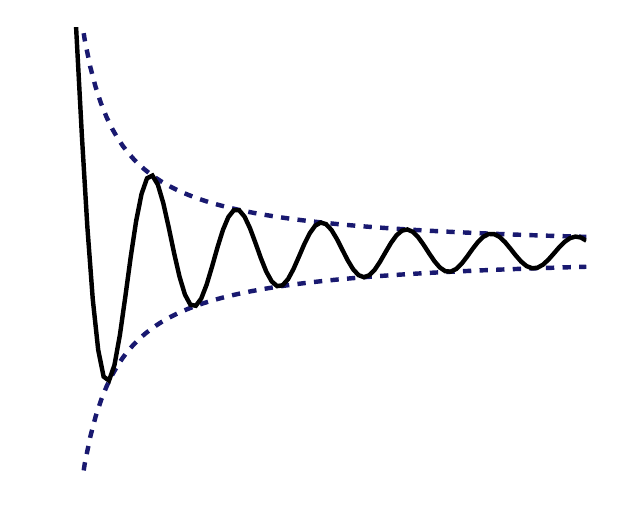
\begin{tikzpicture}[scale=1.0]
        \begin{axis}[
            xmin=0,xmax=20,
            ymin=-0.75,ymax=0.75,
            axis line style={draw=none},
            tick style={draw=none},
            xticklabels=\empty,
            yticklabels=\empty,
        ]
            \addplot[domain=0:20, MidnightBlue, dashed, ultra thick, samples=100] {+1/x};
            \addplot[domain=0:20, MidnightBlue, dashed, ultra thick, samples=100] {-1/x};
            \addplot[domain=0.1:20, black, ultra thick, samples=100] {sin(deg(2*x))/x};
        \end{axis}
    \end{tikzpicture}
}

\chapter{Analysis}
\label{ch:analysis}

\section{Boolean Algebra}

Boolean algebra is the algebra dealing exclusively with the values \textsc{true} and \textsc{false}.

The primary operations of Boolean algebra are \emph{negation} (also called \emph{not}) denoted by $\neg$, \emph{conjunction} (also called \emph{and}) denoted by $\land$, and \emph{disjunction} (also called \emph{or}) denoted by $\lor$.

Since Boolean algebra has only two elements, it is possible to enumerate all variable combinations for a function. This is often done in the form of a truth table --- a table listing the values of variables and the corresponding function value as rows. For example, Table \ref{primary-operations} gives a combined truth table for negation, conjunction, and disjunction. It also serves as the definition of these operations.

\begin{center}
    \captionof{table}{Truth table of primary operations}
    \label{primary-operations}
    \begin{tabularx}{\linewidth}{|X|X|X|X|X|}
        \hline
        \thead{$X$} & \thead{$Y$} & \thead{$\neg X$} & \thead{$X \land Y$} & \thead{$X \lor Y$} \\
        \hline
        \textsc{true} & \textsc{true} & \textsc{false} & \textsc{true} & \textsc{true} \\
        \hline
        \textsc{true}  & \textsc{false} & \textsc{false} & \textsc{false} & \textsc{true} \\
        \hline
        \textsc{false} & \textsc{true} & \textsc{true} & \textsc{false} & \textsc{true} \\
        \hline
        \textsc{false} & \textsc{false} & \textsc{true} & \textsc{false} & \textsc{false} \\
        \hline
    \end{tabularx}
\end{center}

\begin{defn}\label{implies}
    A statement $P$ \emph{implies} (also $\implies$) statement $Q$ if $Q$ is \textsc{true} any time that $P$ is \textsc{true}. When $P$ is \textsc{false}, $Q$ can be \textsc{true} or \textsc{false}. If $P$ is always \textsc{false}, then it implies all statements. $P \implies Q$ is equivalent to $Q \impliedby P$.
\end{defn}

\begin{defn}\label{iff}
    Statement $P$ \emph{if and only if} (also \emph{iff} and $\iff$) statement $Q$ if $P \implies Q$ and $Q \implies P$.
\end{defn}

\begin{thm}{Boolean properties}\label{boolean-algebraic-properties}\proofbreak
    Conjunction and disjunction are commutative:
    \begin{enumerate}
        \item $x \land y = y \land x$
        \item $x \lor y = y \lor x$
    \end{enumerate}

    Conjunction and disjunction are associative:
    \begin{enumerate}
        \item $(x \land y) \land z = x \land (y \land z)$
        \item $(x \lor y) \lor z = x \lor (y \lor z)$
    \end{enumerate}

    Conjunction and disjunction are distributive:
    \begin{enumerate}
        \item $x \land (y \lor z) = (x \land y) \lor (x \land z)$
        \item $x \lor (y \land z) = (x \lor y) \land (x \lor z)$
    \end{enumerate}

    \textup{\textsc{true}} is the identity element (see \ref{identity}) for conjunction and \textup{\textsc{false}} is the identity element for disjunction:
    \begin{enumerate}
        \item $x \land \textup{\textsc{true}} = x$
        \item $x \lor \textup{\textsc{false}} = x$
    \end{enumerate}
\end{thm}

\begin{thm}{Additional properties}\label{additional-boolean-properties}\proofbreak
    \begin{enumerate}
        \item $\neg(\neg x) = x$
        \item $x \land x = x$
        \item $x \lor x = x$
        \item $x \land \neg x = \textup{\textsc{false}}$
        \item $x \lor \neg x = \textup{\textsc{true}}$
    \end{enumerate}
\end{thm}

\begin{thm}{De Morgan's Laws}\label{demorgan-boolean}\proofbreak
    \begin{enumerate}
        \item $\neg(x \land y) = (\neg x) \lor (\neg y)$
        \item $\neg(x \lor y) = (\neg x) \land (\neg y)$
    \end{enumerate}
\end{thm}

\begin{rmk}
    All properties in Theorem \ref{boolean-algebraic-properties}, Theorem \ref{additional-boolean-properties}, and Theorem \ref{demorgan-boolean} can be proved by simply writing out the corresponding truth tables.
\end{rmk}

\section{Sets}

\begin{defn}\label{set}
    A set is an unordered group of distinct elements.
\end{defn}

\begin{exmp}
    $\{1, 2, 3\}$ is a set containing three elements: $1$, $2$, and $3$.
\end{exmp}

\begin{rmk}
    $\{1, 2, 3, 3\}$ is also set containing three elements, since the elements of a set are distinct.
\end{rmk}

\begin{defn}\label{empty-set}
    The empty set (denoted $\emptyset$) is the unique set having no elements.
\end{defn}

One of the most fundamental operations of sets is the ``element of'' operation, denoted by $\in$. $x \in X$ is \textsc{true} precisely when $x$ is an element of the set $X$. Note that sets can be elements of other sets. $x \notin X$ is used to denote ``not an element of''.

\begin{exmp}
    $\left\{\{1, 2\}, \{\}\right\}$ is a set containing two elements: the set $\{1, 2\}$, and the empty set.
\end{exmp}

Set comprehensions, or set builder notation, is a method of precisely defining a set. It can take various forms, such as enumerating all (or implying such) the elements of a set (e.g. $\{1, 2\}$ or $\{1, 2, \ldots, 5\}$). Or it can be used to build a set from another, such as $\left\{2n \compbar n \in \N\right\}$, which says make a set by taking every natural number and doubling it --- these are, of course, the even natural numbers. Set comprehensions can be made more complicated by including a predicate, for example $\left\{n \in \N \compbar n \neq n^2 \right\}$ --- all natural numbers which are not their own square.

Two sets are equal when they contain precisely the same elements. For example, if we let $A = \{1, 1, 5, 2\}$ and $B = \{2, 2, 2, 1, 5\}$, then $A = B$ since for every element $x$ in $A$, $x$ is also in $B$ and vice versa.

\begin{defn}\label{subset}
    A set $T$ is a \emph{subset} of a set $S$ when every element of $T$ is also an element of $S$. This relationship is denoted $T \subseteq S$. $S$ is also referred to as a \emph{super set} of $T$.
\end{defn}

\begin{exmp}
    $\{1, 2, 3\}$ is a subset of $\{1, 2, 3\}$.
\end{exmp}

\begin{rmk}
    If a set $A$ is a subset of set $B$, and $B$ is a subset of $A$, then the sets must be equal. Showing that $A \subseteq B$ and $B \subseteq A$ is a common way to prove that two sets are equal.
\end{rmk}

\begin{defn}\label{proper-subset}
    A set $T$ is a \emph{proper subset} of a set $S$ when every element of $T$ is also an element of $S$, but not vice versa --- that is, the sets are not equal. This relationship is denoted $T \subset S$.
\end{defn}

\begin{exmp}
    $\{1\}$ is a proper subset of $\{1, 2, 3\}$.
\end{exmp}

\begin{defn}\label{intersection}
    The intersection of sets $A$ and $B$ is the set $\left\{x \compbar x \in A \land x \in B \right\}$. It is denoted by $A \intersection B$.
\end{defn}

\begin{exmp}
    $\{1, 2, 3, 4\} \intersection \{3, 4, 5\} = \{3, 4\}$.
\end{exmp}

\begin{defn}
    The union of sets $A$ and $B$ is the set $\left\{x \compbar x \in A \lor x \in B\right\}$. It is denoted by $A \union B$.
\end{defn}

\begin{exmp}
    $\{1, 2, 3, 4\} \union \{3, 4, 5\} = \{1, 2, 3, 4, 5\}$.
\end{exmp}

\begin{rmk}
    If $A$ and $B$ are sets, then $(A \intersection B) \subseteq (A \union B)$. $A = B$ if and only if $(A \intersection B) = (A \union B)$.
\end{rmk}

\begin{defn}
    The complement of set $A$ with respect to some super set $U$ is
    \[\complementof{A} = \left\{x \in U \compbar x \notin A\right\}.\]
\end{defn}

\begin{exmp}
    Let $U = \{1, 2, 3, 4, 5\}$, and $A = \{1, 2\}$. Then $\complementof{A} = \{3, 4, 5\}$.
\end{exmp}

\begin{exmp}
    Let $U = \Z$, and $A$ the even numbers. Then $\complementof{A}$ is the set of the odd numbers.
\end{exmp}

\begin{rmk}
    $\complementof{A} \union A = U$. $\complementof{A} \intersection A = \emptyset$.
\end{rmk}

\begin{defn}\label{set-difference}
    The set difference of sets $A$ and  $B$, denoted $A \setminus B$ or $A - B$, is the set containing all elements of $A$ which are not elements of $B$. $A \setminus B = \left\{x \in A \compbar x \notin B\right\}$.
\end{defn}

\begin{defn}\label{symmetric-difference}
    The symmetric difference of sets $A$ and $B$, denoted $A \triangle B$, is defined to be the set $(A \setminus B) \union (B \setminus A)$.
\end{defn}

\begin{rmk}
    $(A \triangle B)' = (A \intersection B)$ when $U = A \union B$.
\end{rmk}

\begin{thm}\label{set-distributive-rule}\proofbreak
    \begin{enumerate}
        \item $A \land (B \lor C) = (A \land B) \lor (A \land C)$
        \item $A \lor (B \land C) = (A \lor B) \land (A \lor C)$
    \end{enumerate}
\end{thm}

\begin{thm}{De Morgan's Laws}\label{demorgan-set}\proofbreak
    \begin{enumerate}
        \item $\complementof{(A \land B)} = \complementof{A} \lor \complementof{B}$
        \item $\complementof{(A \lor B)} = \complementof{A} \land \complementof{B}$
    \end{enumerate}
\end{thm}

\section{Constructions}

The \emph{von Neumann} construction is one of several ways to construct the natural numbers. It defines $0 = \emptyset$, and defines a function (called the \emph{successor} function) $S(a) = a \union \{a\}$ for every set $a$. Along with the axiom of infinity from Zermelo-Fraenkel set theory, this defines the set of natural numbers.

Using this construction, each natural number is the set of all preceding natural numbers:
\begin{itemize}
    \item $0 = \{\}$
    \item $1 = 0 \union \{0\} = \{\{\}\}$
    \item $2 = 1 \union \{1\} = \{\{\}, \{\{\}\}\}$
    \item $3 = 2 \union \{2\} = \{\{\}, \{\{\}\}, \{\{\}, \{\{\}\}\}\}$
\end{itemize}

Notice that for natural numbers $n, m$, the number of elements of $n$ is $n$, and that $n \leq m \iff n \subseteq m$.

While sets are unordered groups of distinct elements, lists (also called $n$-tuples) are ordered groups of elements which are not necessarily distinct. An ordered pair $(a, b)$ is a list of a length two (a tuple), where $a$, and $b$ are elements of some set.

\begin{defn}\label{tuple}
    An ordered pair $(a, b)$ is a tuple of elements of some set.
\end{defn}

Ordered pairs (and $n$-tuples more generally) can be represented as sets themselves --- the pair $(a, b)$ can be represented as the set $\left\{a, \{a, b\}\right\}$.

\begin{defn}\label{cartesian-product}
    The Cartesian product of two sets $A$ and $B$ is denoted $A \times B$. It is equal to $\left\{\left(a, b\right) \compbar a \in A, b \in B \right\}$.
\end{defn}

\section{Binary Operations}

\begin{defn}
    A \emph{binary operation} is a mathematical operation of arity two, where both domains and the codomain are the same set.
\end{defn}

\begin{exmp}
    Addition on $\R$ is a binary operation, as are multiplication and subtraction.
\end{exmp}

\begin{exmp}
    Let $S$ be the set of all functions $f : \R \to \R$. For any $f, g \in S$, let $f \circ g$ be the function in $S$ defined by $(f \circ g)(x) = f(g(x))$. This is a binary operation on $S$, called function composition.
\end{exmp}

\begin{defn}
    A binary operation $\circ$ on a set $S$ is commutative if $x \circ y = y \circ x$ for all $x, y \in S$.
\end{defn}

\begin{defn}
    A binary operation $\circ$ on a set $S$ is associative if $x \circ (y \circ z) = (x \circ y) \circ z$ for all $x, y, z \in S$.
\end{defn}

\begin{defn}\label{identity}
    Let $\circ$ be a binary operation on a set $S$. Then an element $e$ of $S$ is called a left identity if $e \circ a = a$ for all $a$ in $S$, and a right identity if $a \circ e = a$ for all $a$ in $S$. If $e$ is both a left and a right identity, then it is simply an identity.
\end{defn}

\begin{thm}
    Let $\circ$ be a binary operation on a set $S$. If $\circ$ has both a left identity and a right identity, then those identities are the same.
\end{thm}

\begin{proof}
    Let $e_1$ be a left identity for $\circ$ and $e_2$ be a right identity. Then $e_1 = e_1 \circ e_2 = e_2$, so $e_1 = e_2$.
\end{proof}

\begin{cor}
    If a binary operation has both a left identity and a right identity, it has only a single unique identity.
\end{cor}

\begin{defn}
    Let $\circ$ be a binary operation on a set $S$, and $e$ be an identity element. An element $x$ of a set $S$ is \emph{invertible} if there exists some $x' \in S$ such that $x \circ x' = e$. $x'$ is the \emph{inverse} of $x$.
\end{defn}

\begin{thm}
    Let $\circ$ be a binary associative operation on a set $S$, and $u \in S$ be an invertible element. Then for all $x, y \in S$, $(x \circ u = y \circ u) \implies (x = y)$.
\end{thm}

\begin{proof}
    Let $u'$ be the inverse of the invertible element $u$. Then $(x \circ u) = (y \circ u) \implies (x \circ u) \circ u' = (y \circ u) \circ u'$. Since $\circ$ is associative, this implies that $x \circ (u \circ u') = y \circ (u \circ u')$. Since $u \circ u' = e$, we have $x \circ e = y \circ e$, and so $x = y$.
\end{proof}

\begin{cor}
    Let $\circ$ be a binary associative operation on a set $S$, and $u \in S$ be an invertible element. Then for all $x, y \in S$, $(u \circ x = u \circ y) \implies (x = y)$.
\end{cor}

\section{Relations}

\begin{defn}
    A \emph{relation} $R$ on sets $A$ and $B$ is a set of ordered pairs such that $R \subset A \times B$. For $a \in A, b \in B$, we say that $a$ is related to $b$, denoted by $a R b$, if $(a, b) \in R$.
\end{defn}

\begin{exmp}
    Let $A = \{1, 2, 3, 4\}$, and let $R = \{(1, 1), (2, 2), (3, 3), (4, 4)\}$. $R$ is a relation from $A$ to $A$ that states $a \,R\, a$ if and only if $a = a$. That is, $R$ is an example of a typical equality relation.
\end{exmp}

\begin{exmp}
    $<$, $\leq$, $=$, $>$, $\geq$ are all examples of relations.
\end{exmp}

\begin{defn}
    A relation $R$ on a set $X$ is, for all $x, y, z \in X$:
    \begin{itemize}
        \item \emph{Reflexive} if $x R x$.
        \item \emph{Irreflexive} if $\neg(x R x)$.
        \item \emph{Symmetric} if $x R y \iff y R x$.
        \item \emph{Antisymmetric} if $x R y$ and $y R x$ implies $x = y$.
        \item \emph{Transitive} if $x R y$ and $y R z$ implies $x R z$.
    \end{itemize}
\end{defn}

\begin{exmp}\proofbreak
    \begin{itemize}
        \item $\geq$ is a reflexive relation on $\R$.
        \item $<$ is an irreflexive relation on $\R$.
        \item $a \mid b$ is a symmetric relation on $\R$.
        \item $a \mid b$ is an antisymmetric relation on $\N$.
        \item $\leq$ is a transitive relation on $\R$.
    \end{itemize}
\end{exmp}

\begin{defn}\label{equivalence-relation}
    An \emph{equivalence relation} is a \emph{reflexive}, \emph{symmetric}, and \emph{transitive} relation.
\end{defn}

\begin{defn}
    Let $A, B$ be two sets, and let $R$ be a relation from $A$ to $B$. Then the \emph{inverse} of $R$, denoted by $R^{-1}$, is a relation from $B$ to $A$ given by \[R^{-1} \,= \left\{(b, a) \compbar (a, b) \in R \right\}.\]
\end{defn}

\begin{prop}
    Let $A, B$ be sets, and let $R$ be a relation from $A$ to $B$. Then $\left(R^{-1}\right)^{-1} = R$.
\end{prop}

\begin{proof}
    If $R = \emptyset$, then $R^{-1} = \emptyset$, so $\left(R^{-1}\right)^{-1} = R$.

    Let $(a, b) \in R$. Then by definition, we know $(b, a) \in R^{-1}$, so $(a, b) \in \left(R^{-1}\right)^{-1}$. Therefore, $R \subseteq \left(R^{-1}\right)^{-1}$. Now let $(a, b) \in \left(R^{-1}\right)^{-1}$, so it must be that $(b, a) \in R^{-1}$, so $(a, b) \in R$. Therefore, $\left(R^{-1}\right)^{-1} \subseteq R$, so it follows that $R = \left(R^{-1}\right)^{-1}$.
\end{proof}

\begin{defn}\label{partition}
    A \emph{partition} $P$ of a set $X$ is a set of subsets of $X$ such that:
    \begin{itemize}
        \item $\emptyset \notin P$ --- that is, none of those subsets are empty.
        \item $X = \bigcup_{A\in P}A$ --- that is, every element of $X$ is in a subset.
        \item $(\forall A, B \in P) A \neq B \implies A \intersection B = \emptyset$ --- that is, no element of $X$ is in more than one subset.
    \end{itemize}
    Every $p \in P$ is called a \emph{part} of $P$.
\end{defn}

\begin{exmp}
    Let $X = \{1, 2, 3, 4, 5\}$. Then $P = \left\{\{1, 2, 3\}, \{4, 5\}\right\}$ is a partition of $X$ as every element of $X$ is an element of an element of $P$, no element of $X$ is an element of more than one element of $P$, and no element of $P$ is empty.
\end{exmp}

\begin{exmp}
    The empty set has a unique partition --- the empty set.
\end{exmp}

\begin{defn}
    For a non-empty $X$, $P = \{X\}$ is the \emph{trivial} partition of $X$.
\end{defn}

\begin{defn}\label{equivalence-class}
    Let $S$ be a set and $R$ an equivalence relation on $S$. Then the \emph{equivalence class} of an element $a$ in $S$, denoted by $\left[a\right]$, is the set $\left\{x \in S \compbar x R a\right\}$.
\end{defn}

\begin{lemma}\label{equiv-class-non-empty}
    Let $S$ be a set, $R$ be an equivalence relation on $S$, and $a \in S$. Then $a \in [a]$, and so $[a] \neq \emptyset$.
\end{lemma}

\begin{proof}
    By reflexivity, $a R a$, so it follows that $a \in [a]$.
\end{proof}

\begin{lemma}\label{equiv-class-equal}
    Let $S$ be a set, $R$ be an equivalence relation on $S$, and $a, b \in S$. Then $a R b$ if and only if $[a] = [b]$.
\end{lemma}

\begin{proof}\proofbreak
    ($\implies$) Suppose $a R b$, and let $x \in [a]$. Then $x R a$, and so by transitivity $x R b$, so $x \in [b]$. Therefore, $[a] \subseteq [b]$. If $x \in [b]$, then $x R b$. By symmetry, $b R a$, and so by transitivity, $x R a$, implying that $x \in [a]$. Therefore, $[b] \subseteq [a]$, and so $[a] = [b]$.

    ($\impliedby$) Assume that $[a] = [b]$. Let $x \in [a]$. Then $x \in [b]$, $x R a$, and $x R b$. It follows that by symmetry $a R x$, and by transitivity $a R b$.
\end{proof}

\begin{thm}Equivalence classes form a partition\label{equiv-classes-form-partition}\proofbreak
    Let $S$ be a set, and $R$ an equivalence relation on $S$. If $X$ is the set of all equivalence classes of elements in $S$, then $X$ is a partition of $S$.
\end{thm}

\begin{proof}\proofbreak
    \begin{itemize}
        \item By \ref{equiv-class-non-empty}, there is no $p \in X$ such that $p = \emptyset$, so $\emptyset \notin X$.
        \item Since $a \in S \implies a \in \left[a\right]$, we know that $S \subseteq \bigcup_{A\in X}A$. Since $a \in \bigcup_{A\in X}A$ implies that $a \in A$ for some $A \in X$. Therefore, $a \in S$, so we know that $\bigcup_{A\in X}A \subseteq S$. Therefore, $S = \bigcup_{A\in X}A$.
        \item Let $a, b \in S$ such that $\left[a\right] \intersection \left[b\right] \neq \emptyset$. Then there exists some $x \in (\left[a\right] \intersection \left[b\right])$, so $x R a$ and $x R b$. By symmetry $a R x$, and then by transitivity $a R b$. Then by \ref{equiv-class-equal} we have $\left[a\right] = \left[b\right]$. Therefore, $(\forall A, B \in P) A \neq B \implies A \intersection B = \emptyset$.
    \end{itemize}
    By Definition \ref{partition}, $X$ is a partition of $S$.
\end{proof}

\section{Modular Arithmetic}

\begin{defn}\label{divisible}
    Let $a, b$ be integers. Then we say $b$ is \emph{divisible} by $a$ (written $a \mid b$) when $b = an$ for some integer $n$.
\end{defn}

\begin{exmp}\proofbreak
    \begin{itemize}
        \item $2 \mid 6$ since $6 = 2(3)$
        \item $-3 \mid 21$ since $21 = -3(-7)$
        \item $7 \mid {-7}$ since $-7 = 7(-1)$
        \item $4 \mid 0$ since $0 = 4(0)$
        \item $0 \mid 0$ since $0 = 0(0)$
    \end{itemize}
\end{exmp}

\begin{exmp}\proofbreak
    \begin{itemize}
        \item $4 \centernot\mid 6$ (since there is no $n \in Z$ such that $6 = 4n$)
        \item $6 \centernot\mid 3$ (since there is no $n \in Z$ such that $3 = 6n$)
        \item $2 \centernot\mid 3$ (since there is no $n \in Z$ such that $3 = 2n$)
    \end{itemize}
\end{exmp}

\begin{defn}
    An integer $p$ is \emph{prime} when $1 < p$, and for every $x > 0$, $x \mid p$ implies that $x = 1$ or $x = p$.
\end{defn}

\begin{defn}\label{modular-congruence}
    Let $a, b$ be integers, and $m > 1$ be an integer called the \emph{modulus}. Then $a$ and $b$ are said to be \emph{congruent} modulo $m$, written $a \equiv b \pmod m$, when $m\mid(a - b)$.
\end{defn}

\begin{thm}\label{modular-congruence-equivalence}
    Congruence modulo $m$ is an equivalence relation on the integers.
\end{thm}

\begin{proof} Let $a, b, c$ be integers, and $m > 1$ be an integer.

    Since $(a-a) = 0$ and $0 = 0m$, we have $m|(a-a)$, so $a \equiv a \pmod m$.

    As $a \equiv b \pmod m$ implies that $m\mid(a - b)$, there exists some integer $n$ such that $(a - b) = nm$. Since $(b - a) = -nm$, we know $m\mid(b-a)$. This implies that $a \equiv b \pmod m \iff b \equiv a \pmod m$.

    If $a \equiv b \pmod m$, and $b \equiv c \pmod m$, we know that there exists integers $n_1, n_2$ such that $(a-b) = n_1m$ and $(b-c) = n_2m$. Since $(a-c) = (a-b) + (b-c)$, we know $(a-c) = (n_1 + n_2)m$, and so $a \equiv c \pmod m$.

    Since congruence modulo $m$ is reflexive, symmetric, and transitive, it is an equivalence relation on the integers.
\end{proof}

\begin{defn}\label{mod-n}
    Given an integer $n > 1$, the set $\Z/n\Z = \{0, 1, \ldots, n-1\}$ is the \emph{integers modulo $n$}.
\end{defn}

\begin{defn}\label{modulo}
    Let $a$ be an integer. Then $a$ modulo $n$, written $a \bmod n$, is the unique element $b$ of $\Z/n\Z$ such that $a \equiv b \pmod n$.
\end{defn}

\begin{defn}
    $\oplus_n$ is a binary operation on $\Z_n$ defined by $(a \oplus_n b) = (a + b)\bmod n$.
\end{defn}

\begin{defn}
    $\odot_n$ is a binary operation on $\Z_n$ defined by $(a \odot_n b) = (ab)\bmod n$.
\end{defn}

\begin{defn}
    For $x \in \Z/n\Z$, the multiplicative inverse of $x$ (if it exists), denoted by $x^{-1}$, is a number such that $x \odot_n x^{-1} = 1$.
\end{defn}

\begin{prop}
    Let $x \in \Z/n\Z$. Then $x^{-1}$ exists if and only if $\gcdof{x}{n} = 1$.
\end{prop}

\begin{thm}\label{znz-prime-field}
    If $n$ is a prime integer, then every $x \in \Z/n\Z$, where $x \neq 0$, has a multiplicative inverse $x^{-1}$ in $\Z/n\Z$.
\end{thm}

\begin{proof}
    By Corollary \ref{fermat-little-corallary} to Fermat's little theorem, since $n$ is prime and $n$ does not divide $x$ (since $x < n$), we have $x^{n-1} \equiv 1 \pmod n$. Therefore, $x \odot_n x^{n-2} \equiv 1 \pmod n$, so $x^{-1} = x^{n-2} \bmod n$.
\end{proof}

\section{Fermat's little theorem}

\begin{defn}
    For $n, k \in \N$ where $n \geq k \geq 0$, the binomial coefficient is a positive integer denoted by $\binom{n}{k}$. \[\binom{n}{k} = \frac{n!}{k!(n-k)!}.\]
\end{defn}

\begin{thm}{Binomial theorem}\label{binomial-theorem-ref}\proofbreak
    Let $(F, +, \cdot)$ be a field. Then for any $x, y \in F$ and $n \in \Z_{\geq 1}$, \[\left(x + y\right)^n = \sum_{k=0}^n x^ky^{n-k}{\binom{n}{k}}.\]
\end{thm}

\begin{lemma}\label{prime-divisible-combination}
    Let $p$ be a prime number. Then $p$ divides $\binom{p}{k}$ for $0 < k < p$.
\end{lemma}

\begin{proof}
    Since $p$ is prime, it has no positive divisors other than $1$ and $p$. Since $0 < k < p$, neither $k!$ nor $(p-k)!$ has $p$ as a factor. Therefore, $\binom{p}{k} = p\frac{(p-1)!}{k!(p-k)!}$, so $\binom{p}{k}$ must be divisible by $p$.
\end{proof}

\begin{thm}{Fermat's little theorem}\label{fermat-little-theorem}\proofbreak
    Let $p$ be a prime number. Then for all $n \in \N$, $n^p \equiv n \pmod p$.
\end{thm}

\begin{proof}
    If $n = 1$, then $n^p = 1^p = 1$, so $1^p \equiv 1 \pmod p$.

    Assume $n^p \equiv n \pmod p$ for some $n > 0$. By the binomial theorem \ref{binomial-theorem-ref}, $(n+1)^p = \sum_{k=0}^pn^k\binom{p}{k}$. By Lemma \ref{prime-divisible-combination}, we then know that $(n+1)^p = pw + n^p\binom{p}{p} + n^0\binom{p}{0} = pw + n^p + 1$ for some $w \in \Z$. Since $(pw + n^p + 1) - (n + 1) = pw + (n^p - n)$ and by Definition \ref{modular-congruence} $n^p \equiv n \pmod p$ implies that $p \mid (n^p - n)$, it follows that $p \mid \left[(pw + n^p + 1) - (n + 1)\right]$. Therefore, $(n+1)^p \equiv (n+1) \pmod p$.

    By induction, it follows that $n^p \equiv n \pmod p$ for all $n \in \N$.
\end{proof}

\begin{cor}\label{fermat-little-corallary}
    Since $n^p \equiv n \pmod p$, it follows that $n^{p-1} \equiv 1 \pmod p$.
\end{cor}

\section{Fields}

\begin{defn}
    A \emph{field} $(F, +, \cdot)$ is a set $F$ equipped with two binary operations called addition ($+$) and multiplication ($\cdot$), which do not necessarily correspond to addition and multiplication on the real numbers.

    Field axioms:
    \begin{itemize}
        \item Addition and multiplication are commutative.
        \item Addition and multiplication are associative.
        \item Additive and multiplicative identities, denoted $0$ and $1$ respectively.
        \item Every element $x \in F$ has an additive inverse denoted $-x$.
        \item Every element $x \in F$ where $x \neq 0$ has a multiplicative inverse denoted $x^{-1}$ or $1/x$.
        \item Multiplication is distributive over addition.
    \end{itemize}
\end{defn}

\begin{thm}{Field properties}\label{field-properties}\proofbreak
    For every $x, y, z \in F$:
    \begin{enumerate}
        \item $0 \cdot x = 0$
        \item $(-1) \cdot x = -x$
        \item $-(-x) = x$
        \item If $x \neq 0$, $\left(x^{-1}\right)^{-1} = x$
        \item $x \cdot (-y) = -(x\cdot y)$
        \item $(xy)^{-1} = x^{-1}y^{-1}$
        \item $x\cdot(y-z) = x\cdot y - x \cdot z$
        \item $-(x - y) = y - x$
    \end{enumerate}
\end{thm}

\begin{proof}\proofbreak
    \begin{enumerate}
        \item $0 \cdot x + 0 \cdot x = (0 + 0) \cdot x = 0 \cdot x$. Since the additive identity is unique, this implies that $0 \cdot x = 0$.
        \item $(-1) \cdot x + x = (-1) \cdot x + 1 \cdot x = (-1 + 1) \cdot x = 0 \cdot x = 0$. Therefore, $(-1) \cdot x = -x$.
        \item Let $w = -x$, then $x + w = 0$. Therefore, $x = -w$, and so $x = -(-x)$.
        \item Let $w = x^{-1}$, then $wx = 1 = xw$, so $x = w^{-1}$. Therefore, $x = w^{-1}$, and so $(x^{-1})^{-1} = w^{-1} = w$.
        \item $x \cdot (-y) + xy = x\cdot(-y + y) = x\cdot 0 = 0$.
        \item Let $(xy)(x^{-1}y^{-1}) = (yx)(x^{-1}y^{-1}) = y(xx^{-1})y^{-1} = yy^{-1} = 1$. Since the multiplicative identity is unique, $(xy)^{-1} = x^{-1}y^{-1}$.
        \item $x \cdot (y-z) = x \cdot (y + (-1)z) = x\cdot y + x \cdot (-1)z = xy - xz$.
        \item Since $(x - y) + (y-x) = x + (-y + y) - x = x - x = 0$, we know $-(x - y) = (y - x)$.
    \end{enumerate}
\end{proof}

\begin{defn}
    Let $F$ be a field, and let $x \in F$ and $n \in Z$, $n \geq 0$. Then we recursively define
    \[x^n =
        \begin{dcases}
            1, & n = 0 \\
            x \cdot x^{n-1}, & n > 0
        \end{dcases}.
    \]
\end{defn}

\section{Ordered Fields}

\begin{defn}
    An \emph{ordered field} is a field $(F, +, \cdot)$ together with a subset $F^+ \subset F$ such that\begin{itemize}
        \item For all $x, y \in F^+$, both $x + y$ and $x \cdot y$ are in $F^+$.
        \item (Trichotomy) For all $x \in F$, exactly one of $x \in F^+$, $-x \in F^+$, and $x = 0$ is true.
    \end{itemize}
\end{defn}

If $(F, F^+)$ is an ordered field and $x \in F$, we say $x$ is positive (or $x > 0$) if $x \in F+$.

\begin{defn}
    For elements $x, y$ in an ordered field, we say $x > y$ (or $y < x$) if $x - y > 0$, and $x \geq y$ (or $y \leq x$) if $x = y \lor x > y$.
\end{defn}

\begin{thm} For all $x, y, z, w \in F$, where $F$ is an ordered field:
    \begin{enumerate}
        \item $(x < y) \land (y < z) \implies (x < z)$.
        \item $(x < y) \land (z < w) \implies x + z < y + w$.
        \item $(x > 0) \land (y < 0) \implies xy < 0$.
        \item $(x < 0) \land (y < 0) \implies xy > 0$.
        \item $x \neq 0 \implies x^2 > 0$.
    \end{enumerate}
\end{thm}

\begin{proof}\proofbreak
    \begin{enumerate}
        \item $x < y \land y < z$ implies that $y - x > 0$ and $z - y > 0$. Therefore, $(y - x) + (z - y) = z - x > 0$, so $x < z$.
        \item $x < y \land z < w$ implies that $y - x > 0$ and $w - z > 0$. Therefore, $(y - x) + (w - z) = (y + w) - (x + z) > 0$, so $x + z < y + w$.
        \item $(x > 0) \land (y < 0)$ implies that $-y > 0$. Since $x(-y) > 0$ and $x(-y) = -(xy)$, it follows that $xy < 0$.
        \item $(x < 0) \land (y < 0)$ implies that $(-x)(-y) > 0$. Since $(-x)(-y) = -(-xy) = -(-xy) + (xy  + (-xy)) = (-xy) - (-xy) + xy = 0 + xy = xy$, it follows that $xy > 0$.
        \item If $x > 0$, then $x^2 > 0$. If $x < 0$, then $-x > 0$, so $(-x)^2 > 0$. Since $(-x)(-x) = x^2$, it follows that $x^2 > 0$.
    \end{enumerate}
\end{proof}

\begin{prop}\label{trichotomy-exclusion}
    Let $(F, F^+)$ be an ordered field, and $x, y \in F$. Then at most one of the following is true: $x < y$, $x > y$.
\end{prop}

\begin{proof}
    For the sake of contradiction, assume that $x < y$ and $y > x$. Since $x < y$, we know $y - x > 0$, so $(y - x) \in F^+$. Since $x > y$, we know that $y - x < 0$, so $(y - x) \in F^-$. This contradicts trichotomy, $x < y \land y > x$ cannot be true.
\end{proof}

\begin{prop}\label{greater-than-ratio}
    Let $(F, F^+)$ be an ordered field, and let $x, y \in F^{+}$. Then $x > y$ if and only if $\frac{x}{y} > 1$.
\end{prop}

\begin{proof}\proofbreak
    ($\implies$) If $x > y$, by definition $x - y > 0$. Therefore, $\frac{x}{y} - \frac{y}{y} > 0$, so $\frac{x}{y} - 1 > 0$. This implies that $\frac{x}{y} > 1$.

    ($\impliedby$) If $\frac{x}{y} > 1$, we know that $\frac{x}{y} - 1 > 0$, so it follows that $x - y > 0$. Therefore, we have $x > y$.
\end{proof}

\begin{prop}\label{average-in-between}
    Let $F$ be an ordered field, and $x, y \in F$ with $x < y$. Then $x < \frac{x+y}{2} < y$.
\end{prop}

\begin{proof}
    Since $x < y$, we know that $x + x < x + y$, so $(x + y) - 2x > 0$. Then $\frac{x+y}{2} - x > 0$, so $x < \frac{x+y}{2}$. Similarly, since $x < y$ we know that $x + y < y + y$, so $2y - (x + y) > 0$. Then we have $y - \frac{x + y}{2} > 0$, so $\frac{x + y}{2} < y$. Therefore, $x < \frac{x+y}{2} < y$.
\end{proof}

\begin{prop}\label{multiplicative-inequality-one}
    Let $F$ be an ordered field, and let $a, b, x \in F^+$ such that $a < b$. Then $ax < bx$.
\end{prop}

\begin{proof}
    Since $a < b$, by definition $b - a > 0$. Since $x > 0$, it follows that $x(b-a) > 0$, and so $xb - xa > 0$. Therefore, $ax < bx$ by definition.
\end{proof}

\begin{prop}\label{multiplicative-inequality-two}
    Let $F$ be an ordered field, and let $a, b, c, d \in F^+$ such that $a < b$ and $c < d$. Then $ac < bd$.
\end{prop}

\begin{proof}
    By Proposition \ref{multiplicative-inequality-one}, we know that $ac < bc$, and similarly that $bc < bd$. It follows by transitivity that $ac < bd$.
\end{proof}

\begin{prop}\label{square-is-positive-or-zero}
    Let $F$ be an ordered field, and $x \in F$. Then $x^2 \geq 0$, and $x^2 = 0$ if and only if $x = 0$.
\end{prop}

\begin{proof}
    If
    \begin{itemize}
        \item $x = 0$, then $x^2 = 0(0) = 0$,
        \item $x > 0$, then $x^2 \in F^+$, and so $x^2 > 0$,
        \item $x < 0$, then $(-x)^2 \in F^+$, and since $(-x)^2 = (-1)^2x^2 = x^2$, it follows that $x^2 > 0$.
    \end{itemize}
\end{proof}

\section{Real Numbers}

\begin{defn}
    A \emph{sequence} in a set $X$ is a function $f: \Z_{\geq k} \to X$.
\end{defn}

\begin{exmp}
    Let $f: \Z_{\geq 3} \to Q$ be the function given by $f(n) = \frac{(-1)^n}{n}$.
\end{exmp}

\begin{defn}
    Let $F$ be an ordered field, and $f$ a sequence in $F$. Then we say that $f$ \emph{converges} to some \emph{limit} $x \in F$ if, for every open interval $(a, b) \in F$ containing $x$, there exists $N \in Z_{\geq k}$ such that $f(n) \subseteq (a, b)$ for every $n \geq N$.
\end{defn}

\begin{thm}
    If a sequence $f$ in an ordered field $F$ is convergent, it has a unique limit.
\end{thm}

\begin{proof}
    Assume that a convergent sequence $f$ converges to two distinct limits, $L_1, L_2 \in F$. Since $L_1 \neq L_2$, one must be greater than the other, so without loss of generality we will assume that $L_1 < L_2$. By Proposition \ref{average-in-between}, we know that $L_1 < \frac{L_1+L_2}{2} < L_2$. Construct the open intervals $I_1 = (L_1 - 1, \frac{L_1+L_2}{2})$ and $I_1 = (\frac{L_1+L_2}{2}, I_2 + 1)$. Since $f$ converges to both $L_1$ and $L_2$, there must exist some $N_1, N_2 \in \Z$ such that for all $n \geq N_1$ we have $f(n) \in I_1$, and for all $n \geq N_2$ we have $f(n) \in I_2$. Now let $N$ be the largest of $N_1$ and $N_2$. For any $n \geq N$, we have $f(n) \in I_1$ so $f(n) < \frac{L_1+L_2}{2}$, and for any $n \geq N$, we have $f(n) \in I_2$ so $f(n) > \frac{L_1+L_2}{2}$. By Proposition \ref{trichotomy-exclusion}, this is a contradiction, so it must be that $f$ has a distinct limit.
\end{proof}

\begin{defn}
    A \emph{binary search sequence} in an ordered field $F$ is $\left\{[a_n, b_n]\right\}_{n \geq k}$ with $a_n, b_ \in F$ satisfying $[a_{n+1}, b_{n+1}] \subseteq [a_n, b_n]$ and $b_{n+1}-a_{n+1} = \frac{1}{2}(b_n - a_n)$.
\end{defn}

\begin{defn}
    A binary search sequence \emph{converges} to some $x \in F$ if for all $n \geq k$, $\left\{[a_n, b_n]\right\}$ contains $x$.
\end{defn}

\begin{defn}
    An ordered field $F$ is \emph{complete} if every binary search sequence converges to a unique element of $F$.
\end{defn}

\begin{defn}
    Any complete ordered field is a model for the real numbers.
\end{defn}

\begin{rmk}
    Any two complete ordered fields are isomorphic.
\end{rmk}

\begin{thm}\label{archimedean-property}
    The Archimedean property states that for any $x, y \in \R^{+}$, there exists $n \in \Z_{\geq 1}$ such that $nx > y$.
\end{thm}

\begin{proof}
    For the sake of contradiction, assume there exists some $x, y \in \R^{+}$ such that there is no $n \in \Z$ such that $nx > y$. Therefore, there is some $z \in \R$ where $z = y/x$ such that $z \geq n$ for all $n \in \Z$. Since $2^k \in \Z$ for all $k \in \Z$, it follows that $\frac{z}{2^k} \geq 1$ by Proposition \ref{greater-than-ratio}.

    Now consider the binary search sequence $f(k) = \left\{[0, \frac{z}{2^k}]\right\}_{k \geq 0}$. It is clear that $0 \in f(k)$ for all $k \in \Z_{\geq 0}$, however since $\frac{z}{2^k} \geq 1$, we also have that the $1 \in f(k)$ for all $k \in \Z_{\geq 0}$. This would imply that the binary search sequence converges to both $0$ and $1$, which contradicts the definition of the real numbers, so it follows that there is no such $z \in \R$.
\end{proof}

\begin{cor}
    Suppose $x \in \R$ satisfies $0 \leq x \leq \frac{1}{n}$ for every $n \in \Z_{\geq 1}$. Then $x$ must be zero.
\end{cor}

\begin{proof}
    Assume, for the sake of contradiction, that $x \neq 0$. Then by the Archimedean property \ref{archimedean-property}, there exists $n \in \Z_{\geq 1}$ such that $nx > 1$, and so $x > \frac{1}{n}$ by Proposition \ref{greater-than-ratio}. This is a contradiction, and so $x = 0$.
\end{proof}

\begin{thm}\label{bernoullis-inequality}Bernoulli's inequality\proofbreak
    Let $n \in \Z$, $x \in \R$ such that $n \geq 0$ and $x \geq -1$. Then \[(1 + x)^n \geq 1 + nx.\]
\end{thm}

\begin{proof}
    We will proceed by induction on $n$. For $n=0$, we have $(1 + x)^0 = 1$, and $1 + 0x = 1$, and so the base case is true since $1 \geq 1$.

    Assume that $(1 + x)^n \geq 1 + nx$ for some $n \geq 0$. Then
    \begin{align*}
        (1 + x)^{n+1} &= (1 + x)(1 + x)^n \\
        &= (1 + x)^n + x(1 + x)^n.
    \end{align*}
    Since $(1 + x)^n \geq 1 + nx$, we then have
    \begin{align*}
        (1 + x)^{n+1} &= (1 + x)^n + x(1 + x)^n \\
        &\geq 1 + nx + x(1 + nx) \\
        &= 1 + (n+1)x + nx^2
    \end{align*}
    Note that $x^2 \in \R^+$ by Proposition \ref{square-is-positive-or-zero}, and so $nx^2 \geq 0$. It follows that $1 + (n+1)x + nx^2 \geq 1 + (n+1)x$. Therefore, $(1 + x)^{n+1} \geq 1 + (n+1)x$ by transitivity, and so the induction is complete.
\end{proof}

\begin{lemma}\label{geometric-progression}
    For $r \neq 1$ and $n \in \Z_{\geq 1}$, \[1 + r + r^2 + \cdots + r^{n-1} = \frac{1-r^n}{1-r}.\]
\end{lemma}

\begin{proof}
    We will prove this by induction. For the base case, let $n = 1$. Since $r^0 = 1$, and $\frac{1-r^1}{1-r} = 1$, the base case is true.

    Assume that $1 + r + r^n + \cdots + r^{n-1} = \frac{1-r^n}{1-r}$ for some $n \geq 1$. Then $1 + r + r^n + \cdots + r^{n-1} + r^n = \frac{1-r^n}{1-r} + r^n = \frac{1-r^n}{1-r} + \frac{r^n - r^{n+1}}{1-r}$, so it follows that $1 + r + r^n + \cdots + r^{n-1} + r^n = \frac   {1-r^{n+1}}{1-r}$.

    By the induction principle, it follows that the lemma is true for all $n \geq 1$.
\end{proof}

\begin{lemma}\label{freshmans-reality}
    Let $a, b \in \R$ and $n \in \Z_{\geq 1}$. Then \[b^n - a^n = (b - a)\sum_{k=0}^{n-1} b^ka^{n-1-k}.\]
\end{lemma}

\begin{proof}
    If $b = a$, then $b - a = b^n - a^n = 0$, so the lemma is true in this case.
    If $a = 0$, then $b^n - a^n = b^n$, and $(b - a)\sum_{k=0}^{n-1} b^ka^{n-1-k} = b\sum_{k=0}^{n-1}b^k = b^n$. Now assume $b \neq a$ and $a \neq 0$, and let $r = \frac{b}{a}$. Then $r \neq 1$, so $1 + r + r^2 + \cdots + r^{n-1} = \frac{1-r^n}{1-r}$ by Lemma \ref{geometric-progression}. It then follows that $r^n-1 = (r-1)\sum_{k=0}^{n-1}r^k$. Notice that $r^n - 1 = \frac{b^n}{a^n} - 1 = b^n - a^n$. Therefore, $b^n - a^n = (b-a)\sum_{k=0}^{n-1}b^ka^{n-1-k}$.
\end{proof}

\begin{lemma}\label{exponent-inequality}
    Let $a, b \in \R^+$ such that $a < b$. Then $a^n < b^n$ for all $n \in \Z_{\geq 1}$.
\end{lemma}

\begin{proof}
    We will prove this by induction on $n$. In the base case $n=1$, we have $a^1 = a$ and $b^1 = b$, and so $a^1 < b^1$.

    Assume that $a^n < b^n$ for some $n \geq 1$. Since $a < b$, it follows by Proposition \ref{multiplicative-inequality-two} that $a^n(a) < b^n(b)$ and so $a^{n+1} < b^{n+1}$.

    Therefore, $a^n < b^n$ for all $n \in \Z_{\geq 1}$.
\end{proof}

\begin{lemma}\label{harmonic-vs-powers-of-two}
    For all $n \in \Z_{\geq 1}$, $\frac{1}{2^n} < \frac{1}{n}.$
\end{lemma}

\begin{proof}
    By Proposition \ref{greater-than-ratio}, $\frac{1}{n} > \frac{1}{2^n}$ if and only if $2^n > n$. We will prove this by induction on $n$. In the base case, $n=1$, we have $2^1 = 2 > 1$.

    Assume that $2^n > n$ for some $n \geq 1$. Then
    \begin{align*}
        2^{n+1} &= 2(2^n) > 2n
        &= n + n \geq n + 1,
    \end{align*}
    so the induction is complete.
\end{proof}

\begin{thm}
    Let $n \in \Z_{\geq 1}$, and let $x \in \R^+$. Then there exists $y \in \R^+$ such that $y^n = x$. We say that $y$ is the $n$th root of $x$ in $\R^+$, and denote $y$ by $\sqrt[n]{x}$ or $x^{1/n}$.
\end{thm}

\begin{proof}\proofbreak
\textbf{Uniqueness.} Suppose $y_1, y_2 \in \R^+$ such that $y_1^n = x$ and $y_2^n = x$. By trichotomy, either $y_1 < y_2$, $y_1 = y_2$, or $y_1 > y_2$. If $y_1 < y_2$, then by Lemma \ref{exponent-inequality} it follows that $y_1^n < y_2^n$. However, this would imply that $x < x$ which is a contradiction. Similarly, $y_1 > y_2$ would imply that $x > x$, and so it must be that $y_1 = y_2$.

\textbf{Existence.} Define a sequence in $\R$ starting with $[a_0, b_0] = [0, 1 + x]$, and for $k \leq 0$ as follows.
\[
    [a_{k+1}, b_{k+1}] =
    \begin{dcases}
        \left[a_k, \frac{a_k+b_k}{2}\right], & x \leq \left(\frac{a_k+b_k}{2}\right)^n \\
        \left[\frac{a_k+b_k}{2}, b_k\right], & x > \left(\frac{a_k+b_k}{2}\right)^n
    \end{dcases}
\]

By induction, this sequence must be a binary search sequence. Note that since $a_0 = 0$, and $a_{k+1} \geq a_k$, we know that $0 \leq a_k$, and so if the sequence converges to a value, that value must be greater than or equal to zero.

Now we will show by induction on $k$ that $(a_k)^n \leq x \leq (b_k)^n$ for all $k \in \N$. In the base case, we want to show that $0^n \leq x \leq (1+x)^n$. Since $0^n = 0$ and $x \in \R^+$, we have $0^n \leq x$. Additionally, by Bernoulli's inequality \ref{bernoullis-inequality}, we have $(1+x)^n \geq 1 + nx$, and since $n \geq 1$ it follows that $(1 + x)^n \geq 1 + x > x$, and so $x \leq (1+x)^n$ as needed.

Assume that $a_k^n \leq x \leq b_k^n$ for some $k \leq 0$. If $x \leq \left(\frac{a_k+b_k}{2}\right)^n$, then $a_{k+1} = a_k$ and so $(a_{k+1})^n \leq x$ by assumption and since $b_{k+1} = \frac{a_k+b_k}{2}$, we trivially have $x \leq (b_{k+1})^n$. Similarly, if $x > \left(\frac{a_k+b_k}{2}\right)^n$ then $a_{k+1} = \frac{a_k+b_k}{2}$ and so trivially $(a_{k+1})^n \leq x$, and $x \leq (b_{k+1})^n$. Therefore, the induction is complete and so $a_k^n \leq x \leq b_k^n$ for all $k \in \N$.

By completeness, this binary search sequence converges to a value $y \in \R$ such that $y \geq 0$. Since $y \in [a_k, b_k]$ for all $k$, we know that $0 \leq a_k \leq y \leq b_k$, and so by Lemma \ref{exponent-inequality} we have $(a_k)^n \leq y^n \leq (b_k)^n$. Therefore,
\[x, y^n \in [(a_k)^n, (b_k)^n] \textrm{ for all } k.\] It follows that
\[\abs{x - y^n} \leq (b_k)^n  - (a_k)^n,\] which by Lemma \ref{freshmans-reality} is equal to
\[(b_k - a_k)\sum_{j=0}^{n-1}(b_k)^j(a_j)^{n-1-j},\] and since $a_k \leq b_k$ this is less than or equal to
\[(b_k - a_k)\sum_{j=0}^{n-1}(b_k)^{n-1} = (b_k-a_k)(n)(b_k)^{n-1}.\]
Since the sequence is a binary search sequence, $(b_k-a_k) = \frac{1}{2^k}(b_0 - a_0)$ and $b_k \leq b_0$ so $(b_k)^{n-1} \leq (b_0)^{n-1}$ by Lemma \ref{exponent-inequality}. It follows that
\[(b_k-a_k)(n)(b_k)^{n-1} \leq \frac{1}{2^k}(b_0 - a_0)(n)(b_0)^{n-1},\] and so by transitivity we have
\[\abs{x - y^n} \leq \frac{1}{2^k}(b_0 - a_0)(n)(b_0)^{n-1},\] which implies that
\[0 \leq \frac{\abs{x - y^n}}{(b_0 - a_0)(n)(b_0)^{n-1}} \leq \frac{1}{2^k}.\] Since $\frac{1}{2^k} < \frac{1}{k}$ for $k \geq 1$ by Lemma \ref{harmonic-vs-powers-of-two}, it follows that $\abs{x - y^n} = 0$ by the Archimedean property \ref{archimedean-property}, and so $y^n = x$.
\end{proof}

\begin{defn}
    Let $x \in \R^+$, and $a, b \in \Z$ with $b > 0$. We define $x^{a/b}$ be to $\left(x^{1/b}\right)^a$.
\end{defn}
